% Options for packages loaded elsewhere
\PassOptionsToPackage{unicode}{hyperref}
\PassOptionsToPackage{hyphens}{url}
%
\documentclass[
]{book}
\title{An Incomplete Accounting of my Master's Thesis Research Thus Far}
\author{Quinn Miller}
\date{2022-04-06}

\usepackage{amsmath,amssymb}
\usepackage{lmodern}
\usepackage{iftex}
\ifPDFTeX
  \usepackage[T1]{fontenc}
  \usepackage[utf8]{inputenc}
  \usepackage{textcomp} % provide euro and other symbols
\else % if luatex or xetex
  \usepackage{unicode-math}
  \defaultfontfeatures{Scale=MatchLowercase}
  \defaultfontfeatures[\rmfamily]{Ligatures=TeX,Scale=1}
\fi
% Use upquote if available, for straight quotes in verbatim environments
\IfFileExists{upquote.sty}{\usepackage{upquote}}{}
\IfFileExists{microtype.sty}{% use microtype if available
  \usepackage[]{microtype}
  \UseMicrotypeSet[protrusion]{basicmath} % disable protrusion for tt fonts
}{}
\makeatletter
\@ifundefined{KOMAClassName}{% if non-KOMA class
  \IfFileExists{parskip.sty}{%
    \usepackage{parskip}
  }{% else
    \setlength{\parindent}{0pt}
    \setlength{\parskip}{6pt plus 2pt minus 1pt}}
}{% if KOMA class
  \KOMAoptions{parskip=half}}
\makeatother
\usepackage{xcolor}
\IfFileExists{xurl.sty}{\usepackage{xurl}}{} % add URL line breaks if available
\IfFileExists{bookmark.sty}{\usepackage{bookmark}}{\usepackage{hyperref}}
\hypersetup{
  pdftitle={An Incomplete Accounting of my Master's Thesis Research Thus Far},
  pdfauthor={Quinn Miller},
  hidelinks,
  pdfcreator={LaTeX via pandoc}}
\urlstyle{same} % disable monospaced font for URLs
\usepackage{color}
\usepackage{fancyvrb}
\newcommand{\VerbBar}{|}
\newcommand{\VERB}{\Verb[commandchars=\\\{\}]}
\DefineVerbatimEnvironment{Highlighting}{Verbatim}{commandchars=\\\{\}}
% Add ',fontsize=\small' for more characters per line
\usepackage{framed}
\definecolor{shadecolor}{RGB}{248,248,248}
\newenvironment{Shaded}{\begin{snugshade}}{\end{snugshade}}
\newcommand{\AlertTok}[1]{\textcolor[rgb]{0.94,0.16,0.16}{#1}}
\newcommand{\AnnotationTok}[1]{\textcolor[rgb]{0.56,0.35,0.01}{\textbf{\textit{#1}}}}
\newcommand{\AttributeTok}[1]{\textcolor[rgb]{0.77,0.63,0.00}{#1}}
\newcommand{\BaseNTok}[1]{\textcolor[rgb]{0.00,0.00,0.81}{#1}}
\newcommand{\BuiltInTok}[1]{#1}
\newcommand{\CharTok}[1]{\textcolor[rgb]{0.31,0.60,0.02}{#1}}
\newcommand{\CommentTok}[1]{\textcolor[rgb]{0.56,0.35,0.01}{\textit{#1}}}
\newcommand{\CommentVarTok}[1]{\textcolor[rgb]{0.56,0.35,0.01}{\textbf{\textit{#1}}}}
\newcommand{\ConstantTok}[1]{\textcolor[rgb]{0.00,0.00,0.00}{#1}}
\newcommand{\ControlFlowTok}[1]{\textcolor[rgb]{0.13,0.29,0.53}{\textbf{#1}}}
\newcommand{\DataTypeTok}[1]{\textcolor[rgb]{0.13,0.29,0.53}{#1}}
\newcommand{\DecValTok}[1]{\textcolor[rgb]{0.00,0.00,0.81}{#1}}
\newcommand{\DocumentationTok}[1]{\textcolor[rgb]{0.56,0.35,0.01}{\textbf{\textit{#1}}}}
\newcommand{\ErrorTok}[1]{\textcolor[rgb]{0.64,0.00,0.00}{\textbf{#1}}}
\newcommand{\ExtensionTok}[1]{#1}
\newcommand{\FloatTok}[1]{\textcolor[rgb]{0.00,0.00,0.81}{#1}}
\newcommand{\FunctionTok}[1]{\textcolor[rgb]{0.00,0.00,0.00}{#1}}
\newcommand{\ImportTok}[1]{#1}
\newcommand{\InformationTok}[1]{\textcolor[rgb]{0.56,0.35,0.01}{\textbf{\textit{#1}}}}
\newcommand{\KeywordTok}[1]{\textcolor[rgb]{0.13,0.29,0.53}{\textbf{#1}}}
\newcommand{\NormalTok}[1]{#1}
\newcommand{\OperatorTok}[1]{\textcolor[rgb]{0.81,0.36,0.00}{\textbf{#1}}}
\newcommand{\OtherTok}[1]{\textcolor[rgb]{0.56,0.35,0.01}{#1}}
\newcommand{\PreprocessorTok}[1]{\textcolor[rgb]{0.56,0.35,0.01}{\textit{#1}}}
\newcommand{\RegionMarkerTok}[1]{#1}
\newcommand{\SpecialCharTok}[1]{\textcolor[rgb]{0.00,0.00,0.00}{#1}}
\newcommand{\SpecialStringTok}[1]{\textcolor[rgb]{0.31,0.60,0.02}{#1}}
\newcommand{\StringTok}[1]{\textcolor[rgb]{0.31,0.60,0.02}{#1}}
\newcommand{\VariableTok}[1]{\textcolor[rgb]{0.00,0.00,0.00}{#1}}
\newcommand{\VerbatimStringTok}[1]{\textcolor[rgb]{0.31,0.60,0.02}{#1}}
\newcommand{\WarningTok}[1]{\textcolor[rgb]{0.56,0.35,0.01}{\textbf{\textit{#1}}}}
\usepackage{longtable,booktabs,array}
\usepackage{calc} % for calculating minipage widths
% Correct order of tables after \paragraph or \subparagraph
\usepackage{etoolbox}
\makeatletter
\patchcmd\longtable{\par}{\if@noskipsec\mbox{}\fi\par}{}{}
\makeatother
% Allow footnotes in longtable head/foot
\IfFileExists{footnotehyper.sty}{\usepackage{footnotehyper}}{\usepackage{footnote}}
\makesavenoteenv{longtable}
\usepackage{graphicx}
\makeatletter
\def\maxwidth{\ifdim\Gin@nat@width>\linewidth\linewidth\else\Gin@nat@width\fi}
\def\maxheight{\ifdim\Gin@nat@height>\textheight\textheight\else\Gin@nat@height\fi}
\makeatother
% Scale images if necessary, so that they will not overflow the page
% margins by default, and it is still possible to overwrite the defaults
% using explicit options in \includegraphics[width, height, ...]{}
\setkeys{Gin}{width=\maxwidth,height=\maxheight,keepaspectratio}
% Set default figure placement to htbp
\makeatletter
\def\fps@figure{htbp}
\makeatother
\setlength{\emergencystretch}{3em} % prevent overfull lines
\providecommand{\tightlist}{%
  \setlength{\itemsep}{0pt}\setlength{\parskip}{0pt}}
\setcounter{secnumdepth}{5}
\usepackage{booktabs}
\usepackage{booktabs}
\usepackage{longtable}
\usepackage{array}
\usepackage{multirow}
\usepackage{wrapfig}
\usepackage{float}
\usepackage{colortbl}
\usepackage{pdflscape}
\usepackage{tabu}
\usepackage{threeparttable}
\usepackage{threeparttablex}
\usepackage[normalem]{ulem}
\usepackage{makecell}
\usepackage{xcolor}
\ifLuaTeX
  \usepackage{selnolig}  % disable illegal ligatures
\fi
\usepackage[]{natbib}
\bibliographystyle{plainnat}

\begin{document}
\maketitle

{
\setcounter{tocdepth}{1}
\tableofcontents
}
\hypertarget{about}{%
\chapter{About}\label{about}}

The western United States is seeing an increase in catastrophic wildfire in virtually all climate types and across a broad range of elevations. Many of these fires burn in forested headwaters that communities rely on for water supply, underscoring the need for a greater understanding of how fire changes streamflow timing and magnitude. Though many studies have examined the hydrologic response to fire, the site-specific nature of this type of research has made it difficult to generalize findings. The 2020 Cameron Peak fire in Colorado burned across a broad elevation gradient, making it an ideal case study for examining how the post-fire impact to streamflow generation varies with temperature, aridity, and seasonal snow cover.

We selected three watersheds---unburned, partially burned, and severely burned---in each of two snow zones: the high-elevation persistent snow zone, and the mid-elevation intermittent snow zone. These watersheds were instrumented to monitor snow accumulation and ablation, rainfall, and stream discharge throughout water year 2021. We compared streamflow responses to rainfall and snowmelt between watersheds to evaluate how burning affected runoff. At high elevations, snowmelt runoff began earlier in the burned watersheds, which experienced greater total flow and lower base flows compared to the unburned watershed. The results were similar for the low elevation sites, though less pronounced for snowmelt runoff. At all elevations, streamflow at the burned sites was more responsive to rainfall, with the low elevation sites exhibiting a much more rapid rise to peak discharge than the high elevation sites. The results demonstrate that the streamflow responses to fire vary between snow zones, indicating a need to account for elevation and snow persistence in post-fire risk assessments.

\hypertarget{methods}{%
\chapter{Methods}\label{methods}}

In each of our study watersheds we collected precipitation data using a tipping bucket rain gauge and continuous stream depth using either a capacitance rod or pressure transducer. We also measured stream discharge monthly from April to November 2021. When measuring discharge, we recorded stream stage manually in order to calibrate the sensor data (Fig. \ref{fig:pics})

\begin{figure}
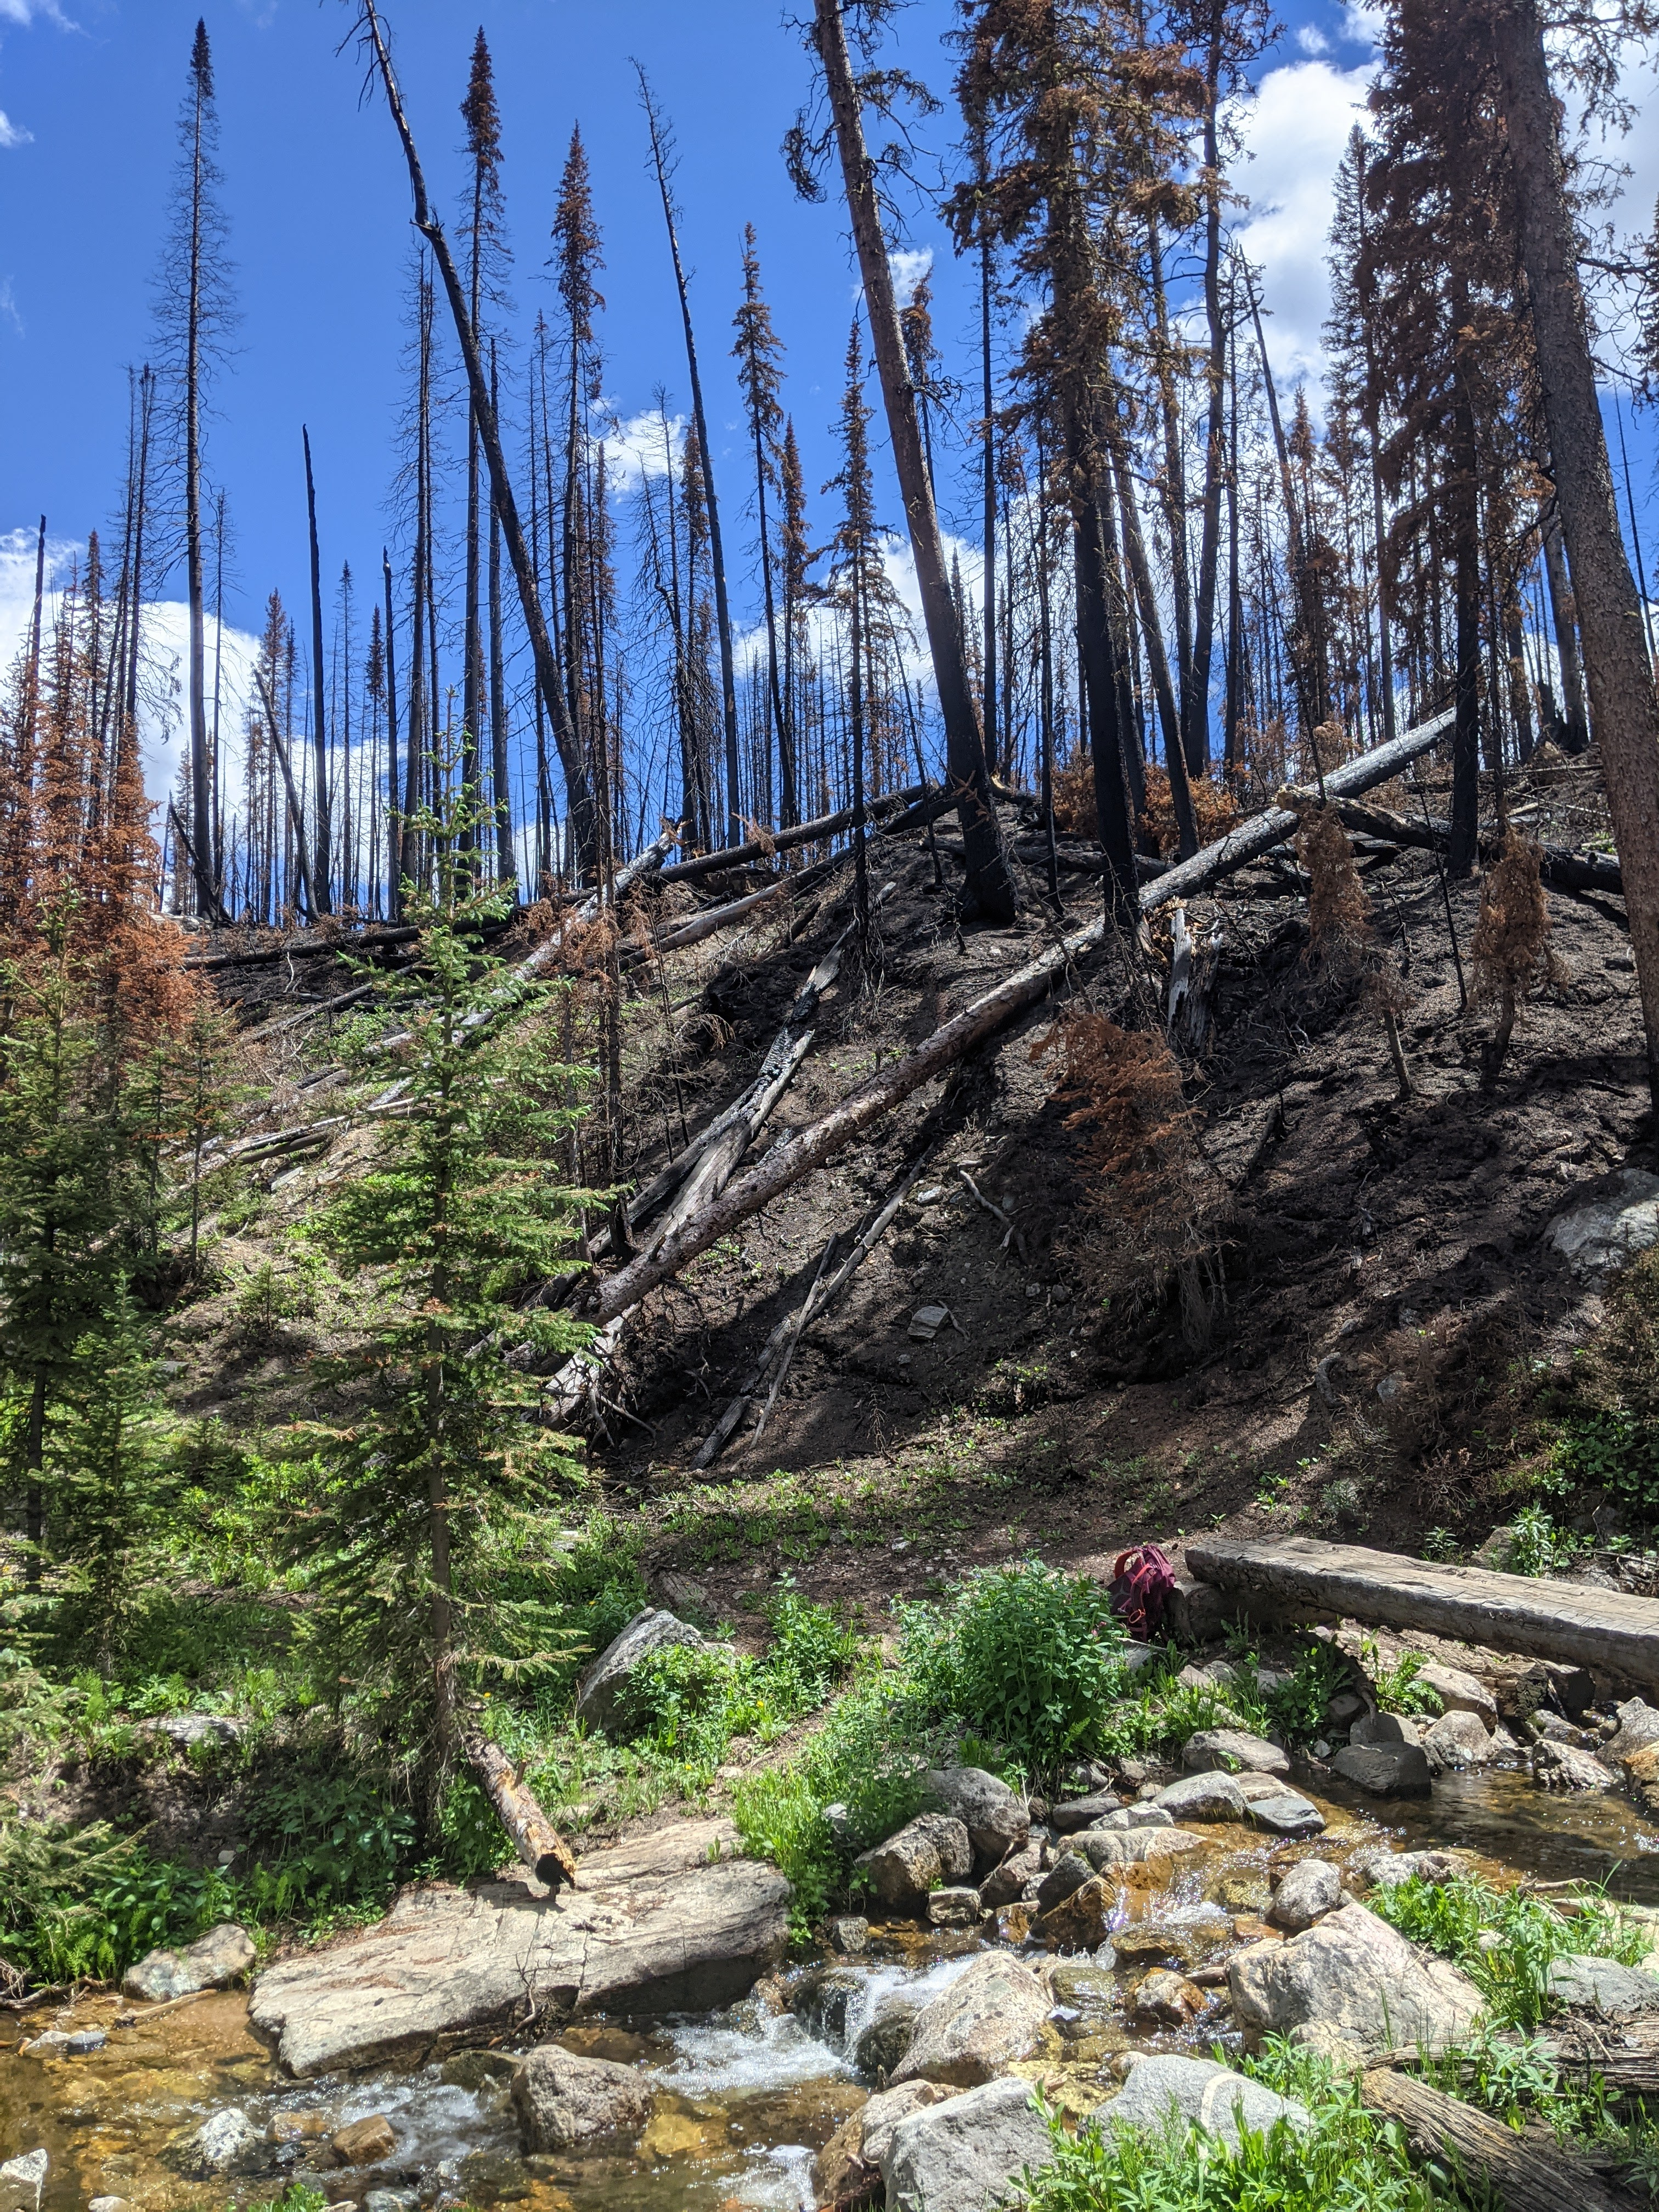
\includegraphics[width=0.5\linewidth]{photos/bl4_bridge} 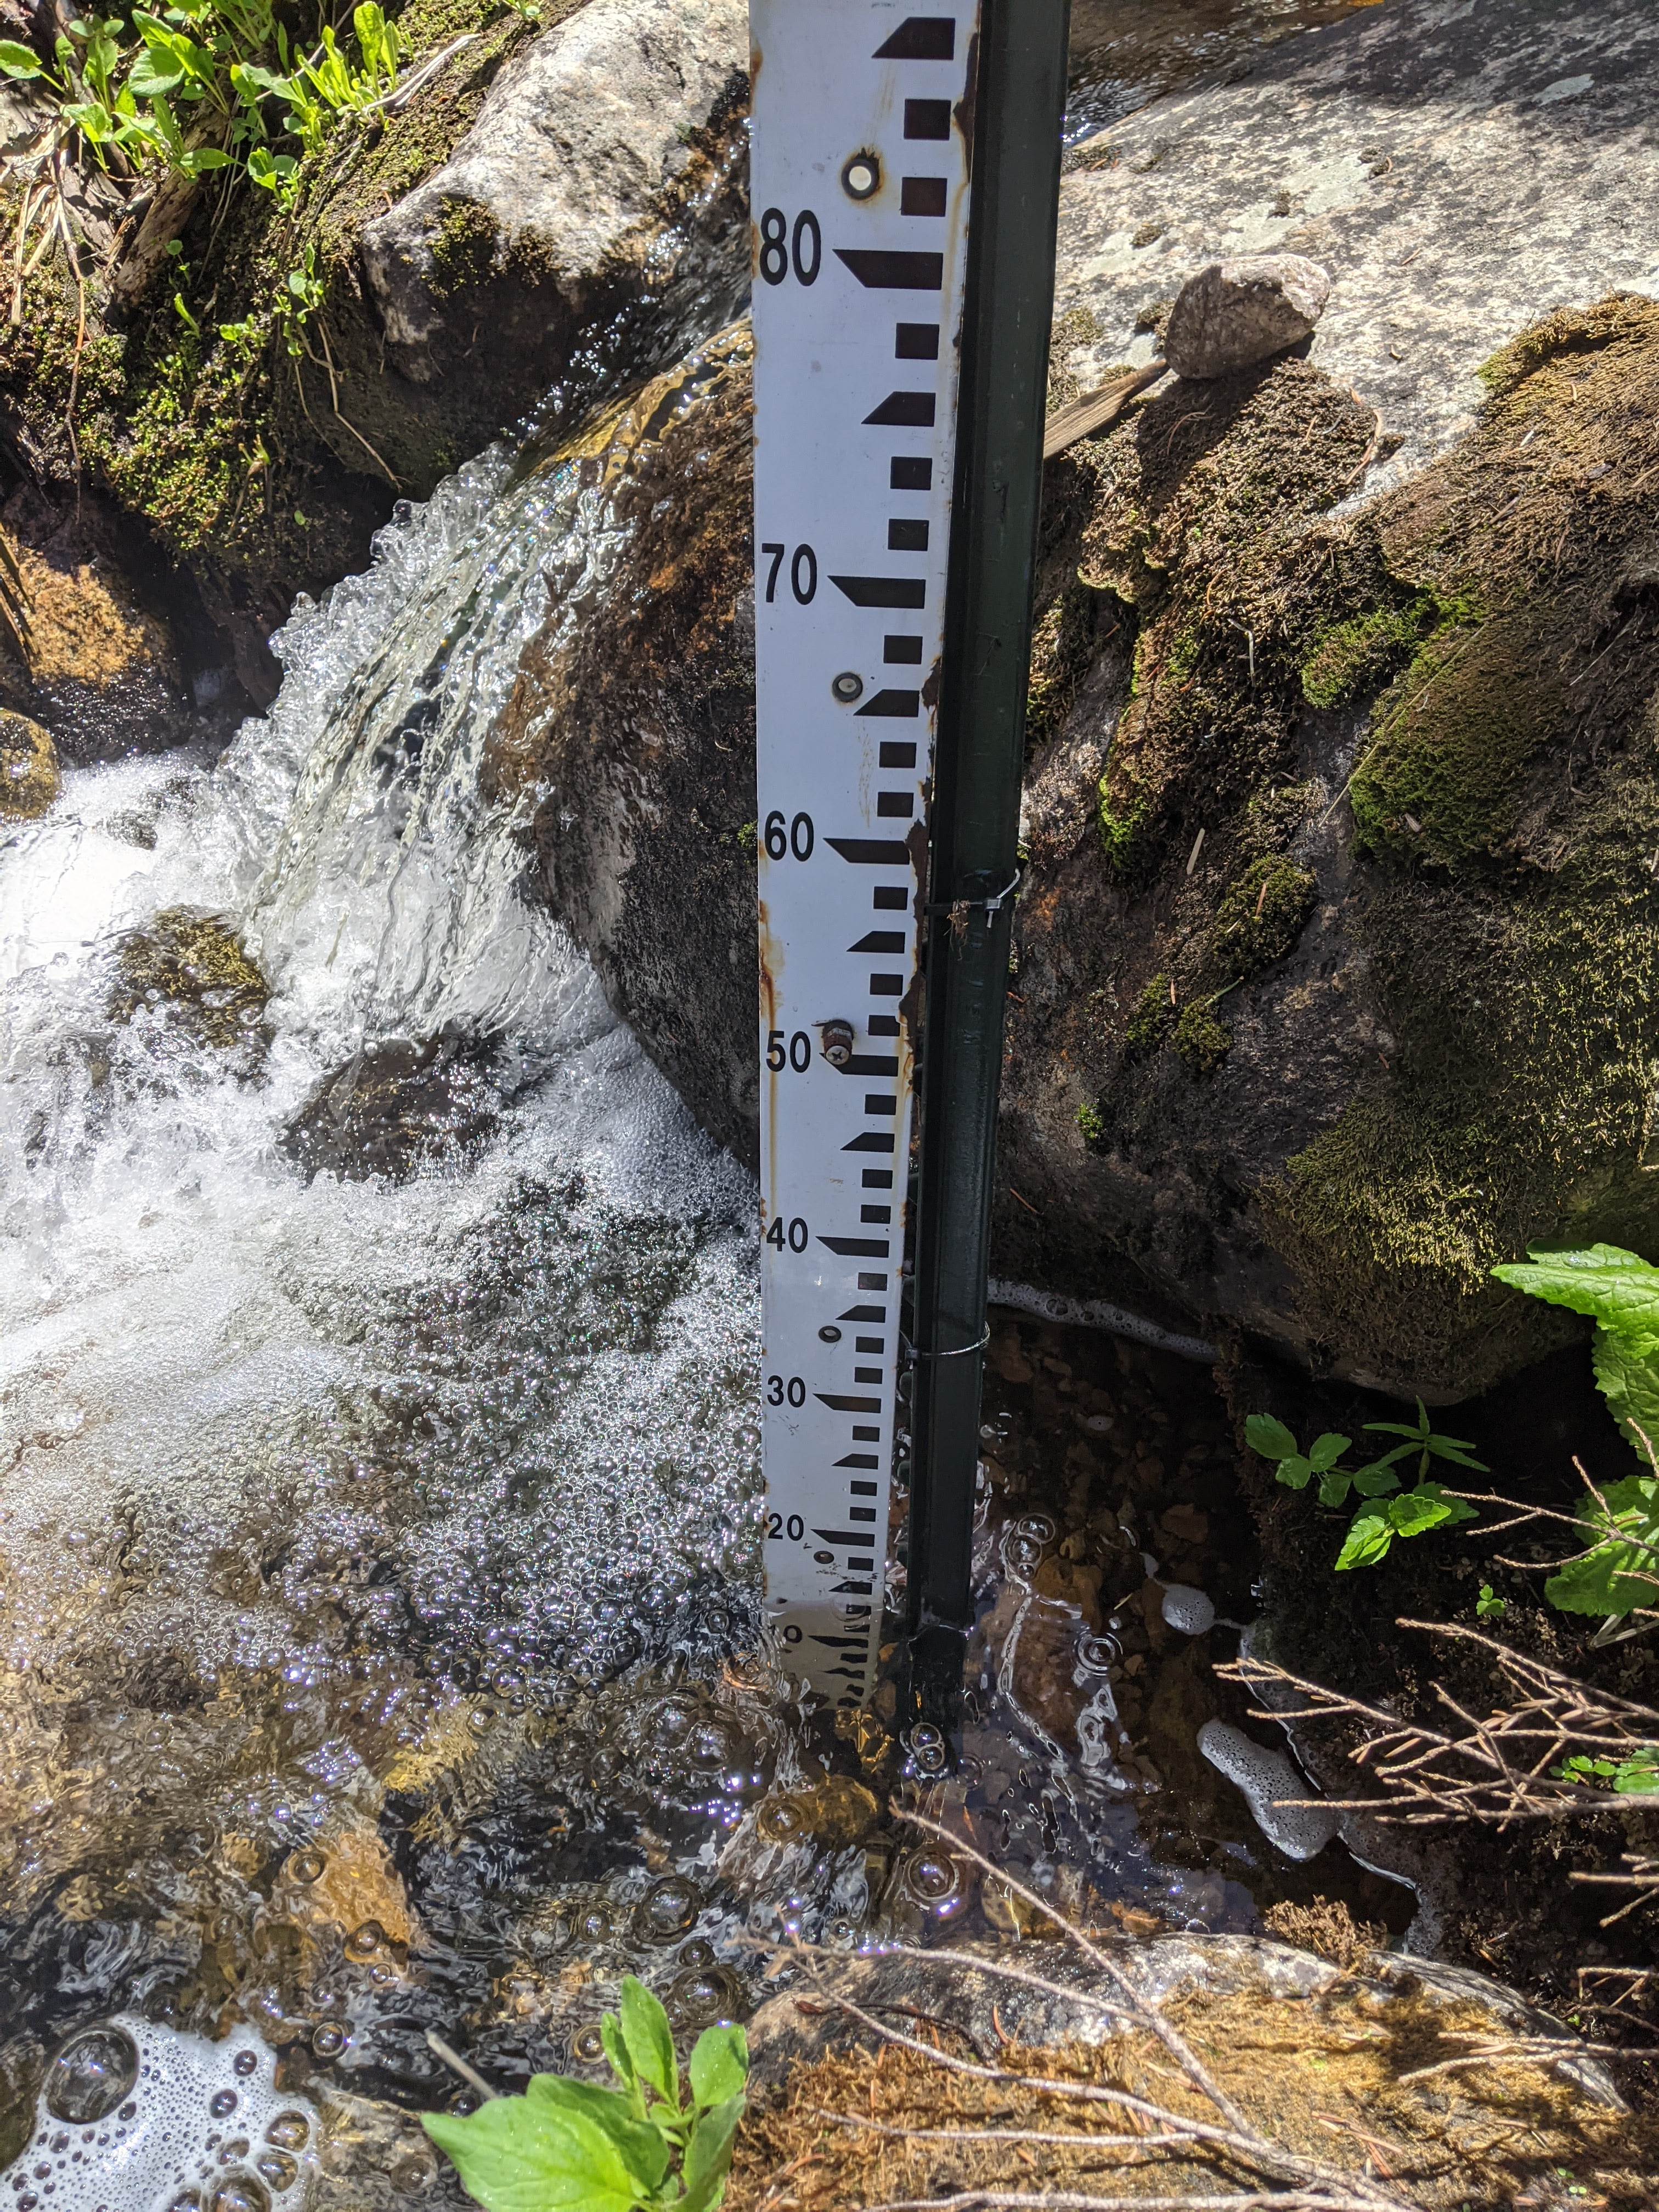
\includegraphics[width=0.5\linewidth]{photos/bl4_sp} \caption{Left: Blue Lake 4 (a tributary to Blue Lake) in June 2021. Right: Staff plate for manual stream stage measurement}\label{fig:pics}
\end{figure}

\hypertarget{site-description}{%
\section{Site Description}\label{site-description}}

For this class report, I will consider two of my field sites-- Blue Lake 4 and Michigan Ditch (Table \ref{tab:descr-tab}). In chapter 4, I will compare our data collection at the Michigan Ditch tributary to the data collected at the nearby USGS Michigan River gage.

\begin{table}

\caption{\label{tab:descr-tab}Properties of the watersheds in this study}
\centering
\begin{tabular}[t]{ccccccc}
\toprule
Watershed & Slope & Aspect & Elevation (m) & Area (sq.km) & Snow Zone & Burn Status\\
\midrule
Bighorn & 19 & SE & 2987.988 & 3.396600 & intermittent & unburned\\
Washout & 33 & E/SE & 2455.392 & 2.695772 & intermittent & partially burned\\
Dry & 18 & E/SE & 2753.429 & 2.520000 & intermittent & severely burned\\
Michigan Ditch & 19 & W/SW & 3462.576 & 1.359900 & persistent & unburned\\
Montgomery & 8 & E/SE & 3070.066 & 1.887741 & persistent & partially burned\\
\addlinespace
Blue Lake 4 & 13 & E/NE & 3065.140 & 0.999655 & persistent & severely burned\\
\bottomrule
\end{tabular}
\end{table}

\hypertarget{data-processing}{%
\chapter{Data Processing}\label{data-processing}}

The goal is to compare rainfall and discharge data in order to compute the following metrics: 1) total quantity of response flow, 2) magnitude of peak response discharge, 3) duration of response, 4) lag to peak time (start time of storm to time of peak discharge), and 5) runoff ratio (depth of Q (mm) divided by the depth of rainfall (mm) for the rain storm associated with the runoff response).

\hypertarget{precipitation}{%
\section{Precipitation}\label{precipitation}}

Before starting this analysis, I identified discrete rainfall events from the tipping bucket rain gauge output using the USDA Rainfall Intensity Summarization Tool (RIST; \citep{ARS2013}). RIST calculated the following metrics for each event: storm duration (hrs), rain depth (mm); maximum intensity (mm h\textsuperscript{−1}) over 5-, 15-, 30-, and 60-min intervals; and erosivity. Because the stage data is recorded every 15 minutes, I'm using the start time of the maximum intensity 15 minute interval as the storm start time. The function below formats the RIST output into the form I want.

\begin{Shaded}
\begin{Highlighting}[]
\CommentTok{\#function to read in rain files}
\NormalTok{rain\_reader }\OtherTok{\textless{}{-}} \ControlFlowTok{function}\NormalTok{(rain\_file)\{}
\NormalTok{  df }\OtherTok{\textless{}{-}}\FunctionTok{read.delim}\NormalTok{(rain\_file, }\AttributeTok{sep =} \StringTok{""}\NormalTok{, }\AttributeTok{header =} \ConstantTok{TRUE}\NormalTok{) }\SpecialCharTok{\%\textgreater{}\%}
  \FunctionTok{select}\NormalTok{(}\SpecialCharTok{{-}}\FunctionTok{c}\NormalTok{(}\DecValTok{1}\NormalTok{,}\DecValTok{3}\SpecialCharTok{:}\DecValTok{7}\NormalTok{))}
\NormalTok{\}}

\CommentTok{\#function to process the storm output }
\NormalTok{rain\_format }\OtherTok{\textless{}{-}} \ControlFlowTok{function}\NormalTok{(rain\_file)\{}
\NormalTok{  df}\OtherTok{\textless{}{-}}\NormalTok{ rain\_file }\SpecialCharTok{\%\textgreater{}\%}
  \FunctionTok{select}\NormalTok{(Max\_15\_start\_date, Max\_15\_start\_time, Precip.in.) }\SpecialCharTok{\%\textgreater{}\%}
  \FunctionTok{rename}\NormalTok{(}\AttributeTok{date =}\DecValTok{1}\NormalTok{, }\AttributeTok{time=}\DecValTok{2}\NormalTok{, }\AttributeTok{p\_in =}\DecValTok{3}\NormalTok{) }\SpecialCharTok{\%\textgreater{}\%}
  \FunctionTok{mutate}\NormalTok{(}\AttributeTok{datetime =} \FunctionTok{paste}\NormalTok{(date, time, }\AttributeTok{sep =} \StringTok{" "}\NormalTok{)) }\SpecialCharTok{\%\textgreater{}\%}
  \FunctionTok{filter}\NormalTok{(}\SpecialCharTok{!}\NormalTok{(p\_in }\SpecialCharTok{==}\DecValTok{0}\NormalTok{)) }\SpecialCharTok{\%\textgreater{}\%}
  \FunctionTok{mutate}\NormalTok{(}\AttributeTok{p\_mm =}\NormalTok{ p\_in}\SpecialCharTok{*}\FloatTok{25.4}\NormalTok{) }\SpecialCharTok{\%\textgreater{}\%}
  \FunctionTok{mutate}\NormalTok{(}\AttributeTok{DateTime =} \FunctionTok{mdy\_hms}\NormalTok{(datetime, }\AttributeTok{tz =} \StringTok{"GMT"}\NormalTok{))  }
\NormalTok{\}}

\CommentTok{\#read in and format michigan ditch and bl4 rain data}
\NormalTok{mich\_rain }\OtherTok{\textless{}{-}} \FunctionTok{rain\_reader}\NormalTok{(}\StringTok{"raw\_sitedata/michiganditch/michigan\_storm.txt"}\NormalTok{)}
\NormalTok{bl4\_rain }\OtherTok{\textless{}{-}} \FunctionTok{rain\_reader}\NormalTok{(}\StringTok{"raw\_sitedata/bl4/bl4\_storm.csv"}\NormalTok{)}

\NormalTok{mich\_storm }\OtherTok{\textless{}{-}} \FunctionTok{rain\_format}\NormalTok{(mich\_rain)}
\NormalTok{bl4\_storm }\OtherTok{\textless{}{-}} \FunctionTok{rain\_format}\NormalTok{(bl4\_rain)}
\end{Highlighting}
\end{Shaded}

\hypertarget{stream-stage}{%
\section{Stream Stage}\label{stream-stage}}

\hypertarget{michigan-ditch}{%
\subsection*{Michigan Ditch}\label{michigan-ditch}}
\addcontentsline{toc}{subsection}{Michigan Ditch}

Michigan Ditch stream stage was recorded by a pressure transducer that doesn't take into account atmospheric pressure, so the data needs to be corrected using barometic data. The continuous stage data is then calibrated according to the manual stage measurements.

\begin{Shaded}
\begin{Highlighting}[]
\CommentTok{\#read in pt data}
\NormalTok{michiganditch\_stage\_pt}\OtherTok{=}\FunctionTok{read\_csv}\NormalTok{(}\StringTok{\textquotesingle{}raw\_sitedata/michiganditch/michiganditch\_stage\_composite\_pt.csv\textquotesingle{}}\NormalTok{, }\AttributeTok{show\_col\_types =} \ConstantTok{FALSE}\NormalTok{) }\SpecialCharTok{\%\textgreater{}\%}
  \FunctionTok{rename}\NormalTok{(}\AttributeTok{Pw\_kPa =} \DecValTok{3}\NormalTok{)}
\NormalTok{michiganditch\_stage\_pt}\SpecialCharTok{$}\NormalTok{DateTime }\OtherTok{=} \FunctionTok{as\_datetime}\NormalTok{(michiganditch\_stage\_pt}\SpecialCharTok{$}\NormalTok{datetime,}\AttributeTok{tz=}\StringTok{"GMT"}\NormalTok{, }\AttributeTok{format=}\StringTok{"\%m/\%d/\%Y \%H:\%M"}\NormalTok{)}

\CommentTok{\#read in baro data}
\NormalTok{michiganditch\_baro}\OtherTok{=}\FunctionTok{read\_csv}\NormalTok{(}\StringTok{\textquotesingle{}raw\_sitedata/michiganditch/michiganditch\_baro\_composite.csv\textquotesingle{}}\NormalTok{, }\AttributeTok{show\_col\_types =} \ConstantTok{FALSE}\NormalTok{) }\SpecialCharTok{\%\textgreater{}\%}
  \FunctionTok{filter}\NormalTok{(}\SpecialCharTok{!}\FunctionTok{is.na}\NormalTok{(Pressure\_kPa)) }\SpecialCharTok{\%\textgreater{}\%}
  \FunctionTok{rename}\NormalTok{(}\AttributeTok{Pa\_kPa =} \DecValTok{2}\NormalTok{)}
\NormalTok{michiganditch\_baro}\SpecialCharTok{$}\NormalTok{DateTime }\OtherTok{=} \FunctionTok{as\_datetime}\NormalTok{(michiganditch\_baro}\SpecialCharTok{$}\NormalTok{datetime,}\AttributeTok{tz=}\StringTok{"GMT"}\NormalTok{, }\AttributeTok{format=}\StringTok{"\%m/\%d/\%Y \%H:\%M"}\NormalTok{)}

\CommentTok{\#join pt and baro and convert to stage in cm}
\NormalTok{mich\_stage }\OtherTok{=} \FunctionTok{full\_join}\NormalTok{(michiganditch\_baro, michiganditch\_stage\_pt, }\AttributeTok{by=}\StringTok{"DateTime"}\NormalTok{,}\AttributeTok{all=}\ConstantTok{TRUE}\NormalTok{) }\SpecialCharTok{\%\textgreater{}\%}
  \FunctionTok{mutate}\NormalTok{(}\AttributeTok{stage\_kPa =}\NormalTok{ Pw\_kPa }\SpecialCharTok{{-}}\NormalTok{ Pa\_kPa) }\SpecialCharTok{\%\textgreater{}\%}
  \FunctionTok{mutate}\NormalTok{(}\AttributeTok{stage\_cm =}\NormalTok{ (stage\_kPa}\SpecialCharTok{*}\FloatTok{101.97162129779}\NormalTok{)}\SpecialCharTok{/}\DecValTok{10}\NormalTok{) }\SpecialCharTok{\%\textgreater{}\%}
  \FunctionTok{select}\NormalTok{(DateTime, stage\_cm)}

\CommentTok{\#read in file with manual stage measurements}
\NormalTok{discharge\_michiganditch}\OtherTok{=}\FunctionTok{read\_csv}\NormalTok{(}\StringTok{\textquotesingle{}raw\_sitedata/michiganditch/discharge\_michiganditch.csv\textquotesingle{}}\NormalTok{, }\AttributeTok{show\_col\_types =} \ConstantTok{FALSE}\NormalTok{)}
\NormalTok{discharge\_michiganditch}\SpecialCharTok{$}\NormalTok{DateTime }\OtherTok{=} \FunctionTok{as.POSIXct}\NormalTok{(discharge\_michiganditch}\SpecialCharTok{$}\NormalTok{datetime,}\AttributeTok{tz=}\StringTok{"GMT"}\NormalTok{,}\AttributeTok{format=}\StringTok{"\%m/\%d/\%Y \%H"}\NormalTok{)}

\CommentTok{\#merge the manual discharge measurements with the sensor time series}
\NormalTok{michditch\_stage}\OtherTok{=}\FunctionTok{full\_join}\NormalTok{(mich\_stage,discharge\_michiganditch,}\AttributeTok{by=}\StringTok{\textquotesingle{}DateTime\textquotesingle{}}\NormalTok{) }\SpecialCharTok{\%\textgreater{}\%}
  \FunctionTok{select}\NormalTok{(}\DecValTok{1}\NormalTok{,}\DecValTok{2}\NormalTok{,}\DecValTok{7}\NormalTok{,}\DecValTok{9}\NormalTok{) }

\CommentTok{\#correct stage based on manual stage measurements}
\NormalTok{michditch\_stage}\OtherTok{\textless{}{-}}\FunctionTok{mutate}\NormalTok{(michditch\_stage, }\AttributeTok{stage\_corr\_cm =}\NormalTok{ stage\_cm)}

\CommentTok{\#offset adjust}
\NormalTok{michditch\_stage}\SpecialCharTok{$}\NormalTok{stage\_corr\_cm}\OtherTok{=}\FunctionTok{ifelse}\NormalTok{(michditch\_stage}\SpecialCharTok{$}\NormalTok{DateTime }\SpecialCharTok{\textgreater{}}\FunctionTok{ymd\_hms}\NormalTok{(}\StringTok{\textquotesingle{}2021{-}06{-}21 10:30:00\textquotesingle{}}\NormalTok{),}
\NormalTok{                                     michditch\_stage}\SpecialCharTok{$}\NormalTok{stage\_corr\_cm}\DecValTok{{-}1}\NormalTok{,michditch\_stage}\SpecialCharTok{$}\NormalTok{stage\_corr\_cm)}

\NormalTok{michditch\_stage}\SpecialCharTok{$}\NormalTok{stage\_corr\_cm}\OtherTok{=}\FunctionTok{ifelse}\NormalTok{(michditch\_stage}\SpecialCharTok{$}\NormalTok{DateTime}\SpecialCharTok{\textgreater{}}\FunctionTok{ymd\_hms}\NormalTok{(}\StringTok{\textquotesingle{}2021{-}08{-}05 11:00:00\textquotesingle{}}\NormalTok{),}
\NormalTok{                                     michditch\_stage}\SpecialCharTok{$}\NormalTok{stage\_corr\_cm}\FloatTok{{-}2.3}\NormalTok{,michditch\_stage}\SpecialCharTok{$}\NormalTok{stage\_corr\_cm)}

\CommentTok{\#delete sensor spikes}
\NormalTok{michditch\_stage }\OtherTok{\textless{}{-}}\NormalTok{ michditch\_stage }\SpecialCharTok{\%\textgreater{}\%}
  \FunctionTok{filter}\NormalTok{(}\SpecialCharTok{!}\NormalTok{(DateTime }\SpecialCharTok{\textless{}} \FunctionTok{ymd\_hms}\NormalTok{(}\StringTok{"2021{-}01{-}10 09:30:00"}\NormalTok{) }\SpecialCharTok{|}
\NormalTok{             DateTime }\SpecialCharTok{==} \FunctionTok{ymd\_hms}\NormalTok{(}\StringTok{"2021{-}06{-}21 09:45:00"}\NormalTok{) }\SpecialCharTok{|}
\NormalTok{             stage\_corr\_cm }\SpecialCharTok{\textless{}=} \DecValTok{0}\NormalTok{))}

\CommentTok{\#plot the sensor and manual stage time series}
\NormalTok{michiganditch}\OtherTok{=}\FunctionTok{ggplot}\NormalTok{()}\SpecialCharTok{+}
  \FunctionTok{geom\_line}\NormalTok{(}\AttributeTok{data=}\NormalTok{michditch\_stage,}\FunctionTok{aes}\NormalTok{(}\AttributeTok{x=}\NormalTok{DateTime,}\AttributeTok{y=}\NormalTok{stage\_corr\_cm))}\SpecialCharTok{+}
  \FunctionTok{geom\_point}\NormalTok{(}\AttributeTok{data=}\NormalTok{michditch\_stage, }\FunctionTok{aes}\NormalTok{(}\AttributeTok{x=}\NormalTok{DateTime,}\AttributeTok{y=}\NormalTok{manual\_stage\_cm),}\AttributeTok{color=}\StringTok{\textquotesingle{}red\textquotesingle{}}\NormalTok{)}\SpecialCharTok{+}
  \FunctionTok{labs}\NormalTok{(}\AttributeTok{x=} \StringTok{"Time"}\NormalTok{, }\AttributeTok{y=} \StringTok{"Stage (cm)"}\NormalTok{) }\SpecialCharTok{+}
  \FunctionTok{theme\_bw}\NormalTok{()}
  
\FunctionTok{ggplotly}\NormalTok{(michiganditch)}
\end{Highlighting}
\end{Shaded}

\begin{verbatim}
## PhantomJS not found. You can install it with webshot::install_phantomjs(). If it is installed, please make sure the phantomjs executable can be found via the PATH variable.
\end{verbatim}

\label{fig:michigan}Michigan Ditch stream stage. The red dots indicate manual stage measurements.

\hypertarget{blue-lake-4}{%
\subsection*{Blue Lake 4}\label{blue-lake-4}}
\addcontentsline{toc}{subsection}{Blue Lake 4}

The Blue Lake data was collected with a capacitance rod, so doesn't need to be corrected for atmospheric pressure.

\begin{Shaded}
\begin{Highlighting}[]
\CommentTok{\#read in file with manual stage measurements}
\NormalTok{discharge\_bl4}\OtherTok{=}\FunctionTok{read\_csv}\NormalTok{(}\StringTok{\textquotesingle{}raw\_sitedata/bl4/discharge\_bl4.csv\textquotesingle{}}\NormalTok{, }\AttributeTok{show\_col\_types =} \ConstantTok{FALSE}\NormalTok{)}
\NormalTok{discharge\_bl4}\SpecialCharTok{$}\NormalTok{DateTime }\OtherTok{=} \FunctionTok{as.POSIXct}\NormalTok{(discharge\_bl4}\SpecialCharTok{$}\NormalTok{datetime,}\AttributeTok{tzone=}\StringTok{"US/Mountain"}\NormalTok{,}\AttributeTok{format=}\StringTok{"\%m/\%d/\%Y \%H"}\NormalTok{)}
\NormalTok{discharge\_bl4[}\DecValTok{1}\SpecialCharTok{:}\DecValTok{2}\NormalTok{,}\DecValTok{10}\NormalTok{] }\OtherTok{=} \FunctionTok{as.POSIXct}\NormalTok{(}\StringTok{\textquotesingle{}2021{-}06{-}01 15:30:00\textquotesingle{}}\NormalTok{)}

\CommentTok{\#read in sensor stage data and format}
\NormalTok{bl4\_stage}\OtherTok{=}\FunctionTok{read\_csv}\NormalTok{(}\StringTok{\textquotesingle{}raw\_sitedata/bl4/bl4\_stage\_composite.csv\textquotesingle{}}\NormalTok{, }\AttributeTok{show\_col\_types =} \ConstantTok{FALSE}\NormalTok{)}
\NormalTok{bl4\_stage}\SpecialCharTok{$}\NormalTok{Date }\OtherTok{=} \FunctionTok{as\_date}\NormalTok{(bl4\_stage}\SpecialCharTok{$}\NormalTok{datetime, }\AttributeTok{format=}\StringTok{"\%m/\%d/\%Y \%H:\%M"}\NormalTok{)}
\NormalTok{bl4\_stage}\SpecialCharTok{$}\NormalTok{DateTime }\OtherTok{=} \FunctionTok{round\_date}\NormalTok{(}\FunctionTok{as\_datetime}\NormalTok{(bl4\_stage}\SpecialCharTok{$}\NormalTok{datetime, }\AttributeTok{format=}\StringTok{"\%m/\%d/\%Y \%H:\%M"}\NormalTok{), }\AttributeTok{unit =} \StringTok{"15 mins"}\NormalTok{)}
\NormalTok{bl4\_stage}\SpecialCharTok{$}\NormalTok{DateTime }\OtherTok{=} \FunctionTok{force\_tz}\NormalTok{(bl4\_stage}\SpecialCharTok{$}\NormalTok{DateTime, }\AttributeTok{tzone =} \StringTok{"US/Mountain"}\NormalTok{ )}
\NormalTok{bl4\_stage }\OtherTok{\textless{}{-}}\FunctionTok{rename}\NormalTok{(bl4\_stage, }\AttributeTok{Stage\_mm =}\NormalTok{ wtrhgt\_\_3)}
\NormalTok{bl4\_stage }\OtherTok{\textless{}{-}}\NormalTok{ bl4\_stage[, }\SpecialCharTok{{-}}\FunctionTok{c}\NormalTok{(}\DecValTok{2}\SpecialCharTok{:}\DecValTok{3}\NormalTok{)]}

\CommentTok{\#convert stage from sensor units to cm}
\NormalTok{bl4\_stage}\SpecialCharTok{$}\NormalTok{Stage\_cm}\OtherTok{=}\NormalTok{bl4\_stage}\SpecialCharTok{$}\NormalTok{Stage\_mm}\SpecialCharTok{/}\DecValTok{10}

\CommentTok{\#merge the manual discharge measurements with the sensor time series}
\NormalTok{bl4\_stage}\OtherTok{=}\FunctionTok{full\_join}\NormalTok{(bl4\_stage,discharge\_bl4,}\AttributeTok{by=}\StringTok{\textquotesingle{}DateTime\textquotesingle{}}\NormalTok{)}

\CommentTok{\#delete bad measurements{-}{-} sensor spikes and other obvious errors}
\NormalTok{bl4\_stage}\OtherTok{\textless{}{-}}\FunctionTok{filter}\NormalTok{(bl4\_stage, datetime.x }\SpecialCharTok{!=} \StringTok{"8/6/2021 8:45"}\NormalTok{)}
\NormalTok{bl4\_stage}\OtherTok{\textless{}{-}}\FunctionTok{filter}\NormalTok{(bl4\_stage, datetime.x }\SpecialCharTok{!=} \StringTok{"6/1/2021 10:33"}\NormalTok{)}
\NormalTok{bl4\_stage}\OtherTok{\textless{}{-}}\FunctionTok{filter}\NormalTok{(bl4\_stage, datetime.x }\SpecialCharTok{!=} \StringTok{"6/1/2021 11:33"}\NormalTok{)}
\NormalTok{bl4\_stage}\OtherTok{\textless{}{-}}\FunctionTok{filter}\NormalTok{(bl4\_stage, datetime.x }\SpecialCharTok{!=} \StringTok{"6/1/2021 12:33"}\NormalTok{)}
\NormalTok{bl4\_stage}\OtherTok{\textless{}{-}}\FunctionTok{filter}\NormalTok{(bl4\_stage, datetime.x }\SpecialCharTok{!=} \StringTok{"6/1/2021 13:33"}\NormalTok{)}

\CommentTok{\#goal is to offset{-}adjust sensor stage to levels of manual stage}
\NormalTok{bl4\_stage}\SpecialCharTok{$}\NormalTok{Stage\_corr\_cm }\OtherTok{=}\NormalTok{ bl4\_stage}\SpecialCharTok{$}\NormalTok{Stage\_cm}
\NormalTok{bl4\_stage}\SpecialCharTok{$}\NormalTok{Stage\_corr\_cm }\OtherTok{=} \FunctionTok{ifelse}\NormalTok{(bl4\_stage}\SpecialCharTok{$}\NormalTok{DateTime }\SpecialCharTok{\textless{}} \StringTok{\textquotesingle{}2021{-}06{-}01 14:30:00\textquotesingle{}}\NormalTok{,}
\NormalTok{                                        bl4\_stage}\SpecialCharTok{$}\NormalTok{Stage\_corr\_cm }\SpecialCharTok{+}\DecValTok{6}\NormalTok{, bl4\_stage}\SpecialCharTok{$}\NormalTok{Stage\_corr\_cm}\SpecialCharTok{+}\DecValTok{2}\NormalTok{)}

\NormalTok{bl4\_stage}\SpecialCharTok{$}\NormalTok{Stage\_corr\_cm }\OtherTok{=} \FunctionTok{ifelse}\NormalTok{(bl4\_stage}\SpecialCharTok{$}\NormalTok{DateTime }\SpecialCharTok{\textgreater{}} \StringTok{\textquotesingle{}2021{-}06{-}11 12:30:00\textquotesingle{}}\NormalTok{,}
\NormalTok{                                         bl4\_stage}\SpecialCharTok{$}\NormalTok{Stage\_corr\_cm }\SpecialCharTok{+}\FloatTok{4.4}\NormalTok{, bl4\_stage}\SpecialCharTok{$}\NormalTok{Stage\_corr\_cm)}

\NormalTok{bl4\_stage}\SpecialCharTok{$}\NormalTok{Stage\_corr\_cm }\OtherTok{=} \FunctionTok{ifelse}\NormalTok{(bl4\_stage}\SpecialCharTok{$}\NormalTok{DateTime }\SpecialCharTok{\textgreater{}} \StringTok{\textquotesingle{}2021{-}07{-}02 13:45:00\textquotesingle{}}\NormalTok{,}
\NormalTok{                                        bl4\_stage}\SpecialCharTok{$}\NormalTok{Stage\_corr\_cm }\SpecialCharTok{+}\FloatTok{0.2}\NormalTok{, bl4\_stage}\SpecialCharTok{$}\NormalTok{Stage\_corr\_cm)}

\NormalTok{bl4\_stage}\SpecialCharTok{$}\NormalTok{Stage\_corr\_cm }\OtherTok{=} \FunctionTok{ifelse}\NormalTok{(bl4\_stage}\SpecialCharTok{$}\NormalTok{DateTime }\SpecialCharTok{\textgreater{}} \StringTok{\textquotesingle{}2021{-}08{-}06 08:30:00\textquotesingle{}}\NormalTok{,}
\NormalTok{                                 bl4\_stage}\SpecialCharTok{$}\NormalTok{Stage\_corr\_cm }\SpecialCharTok{+}\FloatTok{0.5}\NormalTok{, bl4\_stage}\SpecialCharTok{$}\NormalTok{Stage\_corr\_cm)}


\CommentTok{\#plot the sensor and manual stage time series}
\NormalTok{bl4}\OtherTok{=}\FunctionTok{ggplot}\NormalTok{()}\SpecialCharTok{+}\FunctionTok{geom\_line}\NormalTok{(}\AttributeTok{data=}\NormalTok{bl4\_stage,}\FunctionTok{aes}\NormalTok{(}\AttributeTok{x=}\NormalTok{DateTime,}\AttributeTok{y=}\NormalTok{Stage\_corr\_cm))}\SpecialCharTok{+}
  \FunctionTok{geom\_point}\NormalTok{(}\AttributeTok{data=}\NormalTok{bl4\_stage,}\FunctionTok{aes}\NormalTok{(}\AttributeTok{x=}\NormalTok{DateTime,}\AttributeTok{y=}\NormalTok{manual\_stage\_cm),}\AttributeTok{color=}\StringTok{\textquotesingle{}red\textquotesingle{}}\NormalTok{)}\SpecialCharTok{+}
  \FunctionTok{labs}\NormalTok{(}\AttributeTok{x=} \StringTok{"Time"}\NormalTok{, }\AttributeTok{y=} \StringTok{"Stage (cm)"}\NormalTok{) }\SpecialCharTok{+}
  \FunctionTok{theme\_bw}\NormalTok{()}
\FunctionTok{ggplotly}\NormalTok{(bl4)}
\end{Highlighting}
\end{Shaded}

\label{fig:bl4}Bl4 stream stage. The red dots indicate manual stage measurements.

\hypertarget{discharge}{%
\section{Discharge}\label{discharge}}

Rating curves were developed for both sites using JMP statistical software.

\begin{Shaded}
\begin{Highlighting}[]
\CommentTok{\#michigan ditch rc is a sqrt transform of the y axis}
\NormalTok{michditch\_stage}\SpecialCharTok{$}\NormalTok{Discharge\_Ls }\OtherTok{=}\NormalTok{ (}\SpecialCharTok{{-}}\FloatTok{0.218979} \SpecialCharTok{+} \FloatTok{0.3533779}\SpecialCharTok{*}\NormalTok{(michditch\_stage}\SpecialCharTok{$}\NormalTok{stage\_corr\_cm))}\SpecialCharTok{\^{}}\DecValTok{2}
  
\CommentTok{\#plot sensor discharge and manual discharge to make sure rating curve was applied correctly}
\NormalTok{michiganditch}\OtherTok{=}\FunctionTok{ggplot}\NormalTok{(michditch\_stage)}\SpecialCharTok{+}
  \FunctionTok{geom\_line}\NormalTok{(}\FunctionTok{aes}\NormalTok{(}\AttributeTok{x=}\NormalTok{DateTime,}\AttributeTok{y=}\NormalTok{Discharge\_Ls))}\SpecialCharTok{+}
  \FunctionTok{geom\_point}\NormalTok{(}\FunctionTok{aes}\NormalTok{(}\AttributeTok{x=}\NormalTok{DateTime,}\AttributeTok{y=}\NormalTok{discharge\_Ls),}\AttributeTok{color=}\StringTok{\textquotesingle{}red\textquotesingle{}}\NormalTok{)}

\FunctionTok{ggplotly}\NormalTok{(michiganditch)}
\end{Highlighting}
\end{Shaded}

\label{fig:rc}Plots of discharge; Michigan Ditch on the left and Blue Lake 4 on the right.

\begin{Shaded}
\begin{Highlighting}[]
\CommentTok{\#bl4 rc is a gompertz 3p sigmoid curve}
\NormalTok{a}\OtherTok{=}\FloatTok{159.07732}
\NormalTok{b}\OtherTok{=}\FloatTok{0.0997502}
\NormalTok{c}\OtherTok{=}\FloatTok{23.905566}

\NormalTok{bl4\_stage}\SpecialCharTok{$}\NormalTok{Discharge\_Ls }\OtherTok{=}\NormalTok{ a}\SpecialCharTok{*}\FunctionTok{exp}\NormalTok{(}\SpecialCharTok{{-}}\FunctionTok{exp}\NormalTok{(}\SpecialCharTok{{-}}\NormalTok{b}\SpecialCharTok{*}\NormalTok{(bl4\_stage}\SpecialCharTok{$}\NormalTok{Stage\_corr\_cm }\SpecialCharTok{{-}}\NormalTok{ c)))}

\CommentTok{\#plot sensor discharge and manual discharge to make sure rating curve was applied correctly}
\NormalTok{bl4}\OtherTok{=}\FunctionTok{ggplot}\NormalTok{()}\SpecialCharTok{+}\FunctionTok{geom\_line}\NormalTok{(}\AttributeTok{data=}\NormalTok{bl4\_stage,}\FunctionTok{aes}\NormalTok{(}\AttributeTok{x=}\NormalTok{DateTime,}\AttributeTok{y=}\NormalTok{Discharge\_Ls))}\SpecialCharTok{+}
  \FunctionTok{geom\_point}\NormalTok{(}\AttributeTok{data=}\NormalTok{bl4\_stage,}\FunctionTok{aes}\NormalTok{(}\AttributeTok{x=}\NormalTok{DateTime,}\AttributeTok{y=}\NormalTok{discharge\_Ls),}\AttributeTok{color=}\StringTok{\textquotesingle{}red\textquotesingle{}}\NormalTok{)}\SpecialCharTok{+}
  \FunctionTok{xlab}\NormalTok{(}\StringTok{"Time"}\NormalTok{)}\SpecialCharTok{+} \FunctionTok{ylab}\NormalTok{(}\StringTok{"Discharge (L/s)"}\NormalTok{)}\SpecialCharTok{+}
  \FunctionTok{theme\_bw}\NormalTok{()}

\FunctionTok{ggplotly}\NormalTok{(bl4)}
\end{Highlighting}
\end{Shaded}

\label{fig:rc}Plots of discharge; Michigan Ditch on the left and Blue Lake 4 on the right.

\hypertarget{comparison-of-salt-dilution-to-usgs-gage}{%
\chapter{Comparison of Salt Dilution to USGS Gage}\label{comparison-of-salt-dilution-to-usgs-gage}}

You can add parts to organize one or more book chapters together. Parts can be inserted at the top of an .Rmd file, before the first-level chapter heading in that same file.

Add a numbered part: \texttt{\#\ (PART)\ Act\ one\ \{-\}} (followed by \texttt{\#\ A\ chapter})

Add an unnumbered part: \texttt{\#\ (PART\textbackslash{}*)\ Act\ one\ \{-\}} (followed by \texttt{\#\ A\ chapter})

Add an appendix as a special kind of un-numbered part: \texttt{\#\ (APPENDIX)\ Other\ stuff\ \{-\}} (followed by \texttt{\#\ A\ chapter}). Chapters in an appendix are prepended with letters instead of numbers.

\hypertarget{footnotes-and-citations}{%
\chapter{Footnotes and citations}\label{footnotes-and-citations}}

\hypertarget{footnotes}{%
\section{Footnotes}\label{footnotes}}

Footnotes are put inside the square brackets after a caret \texttt{\^{}{[}{]}}. Like this one \footnote{This is a footnote.}.

\hypertarget{citations}{%
\section{Citations}\label{citations}}

Reference items in your bibliography file(s) using \texttt{@key}.

For example, we are using the \textbf{bookdown} package \citep{R-bookdown} (check out the last code chunk in index.Rmd to see how this citation key was added) in this sample book, which was built on top of R Markdown and \textbf{knitr} \citep{xie2015} (this citation was added manually in an external file book.bib).
Note that the \texttt{.bib} files need to be listed in the index.Rmd with the YAML \texttt{bibliography} key.

The RStudio Visual Markdown Editor can also make it easier to insert citations: \url{https://rstudio.github.io/visual-markdown-editing/\#/citations}

  \bibliography{book.bib,packages.bib}

\end{document}
